\documentclass[]{beamer}
\usetheme[color=screen]{UniBern}

%\setbeameroption{show notes}
%\includeonlyframes{current}

\usepackage{lmodern}
\usepackage[english]{babel}
\usepackage{microtype}
\usepackage{textcomp}
\usepackage[backend=biber, style=alphabetic, url=false]{biblatex}
\addbibresource{../../Documents/library.bib}
\usepackage{graphicx}
\usepackage{caption}
	\captionsetup[figure]{labelformat=empty} % No 'figure' in figures
\usepackage{tikz}
	\usetikzlibrary{arrows.meta,shapes}
\usepackage[detect-all=true, range-phrase=--, range-units=single]{siunitx}
\usepackage{csquotes}
\usepackage{animate}
\usepackage{sparklines}
\usepackage{booktabs}
\usepackage[absolute,overlay]{textpos} %for the \source{} command
\usepackage{gitinfo2}
\usepackage{xspace}
\usepackage{todonotes}
	\presetkeys{todonotes}{inline}{} % http://tex.stackexchange.com/a/12331/828
\usepackage{hyperref}

\hypersetup{pdfstartview={Fit}}
\setbeamertemplate{caption}{\insertcaption}
\setbeamertemplate{caption}[numbered]

\newcommand{\imsize}{\linewidth}
\newlength\imagewidth % needed for scalebars
\newlength\imagescale % ditto
\newcommand{\uct}{\si{\micro}CT\xspace}
\newcommand{\uaf}{\si{\micro}AngioFil\xspace}

\newcommand{\source}[1]{%http://tex.stackexchange.com/a/48485/828
	\begin{textblock*}{4cm}(8.7cm,8.6cm)%
		\begin{beamercolorbox}[ht=0.5cm,right]{framesource}%
			\tiny\usebeamerfont{framesource}\usebeamercolor[fg]{framesource} Source: {#1}%
		\end{beamercolorbox}%
	\end{textblock*}%
}

% define unibe color
\definecolor{unibe}{RGB}{156,189,222}

% Biblatex: http://tex.stackexchange.com/a/13076/828
% Format bibliography for beamer
% http://tex.stackexchange.com/a/10686/828
\renewbibmacro{in:}{}
% % http://tex.stackexchange.com/a/13076/828
% \AtEveryBibitem{\clearfield{title}}
% \AtEveryBibitem{\clearfield{journaltitle}}
% \AtEveryBibitem{\clearfield{year}}
% \AtEveryBibitem{\clearfield{pages}}
% \AtEveryBibitem{\clearfield{volume}}
% \AtEveryBibitem{\clearfield{number}}
% %http://tex.stackexchange.com/a/40710/828
% \usepackage{xpatch}
% \xpatchbibmacro{month}{%
%   \printtext[parens]%
% }{%
%   \setunit*{\addperiod\space}%
%   \printtext%
% }{}{} 

\subtitle{Several examples as well as details in lung and brain imaging}
\author[David Haberthür]{David Haberthür \and\tiny Adolfo Odriozola \and Ruslan Hlushchuk \and Valentin Djonov}
\institute{Institute of Anatomy, University of Bern}
\date{February 9, 2017\\Internal Seminar}

\begin{document}
\title[\si{\micro}CT in biological studies]{\si{\micro}CT-imaging at the Institute of Anatomy} % http://tex.stackexchange.com/a/144445/828

\defbeamertemplate{footline}{unibe}
{%
\usebeamercolor[fg]{page number in head/foot}%
	\usebeamerfont{page number in head/foot}%
	\hspace*{\fill}%
	\insertshortauthor%
	\hspace*{\fill}%|\hspace*{\fill}%
	\insertshorttitle%
	\hspace*{\fill}%|\hspace*{\fill}%
	v.~\gitAbbrevHash%
	\hspace*{\fill}%|\hspace*{\fill}%
	\insertframenumber\,/\,\insertpresentationendpage%
	\hspace*{\fill}%
	\vskip2pt%
}
\setbeamertemplate{footline}[unibe]

{%
% No footline on title page: http://tex.stackexchange.com/a/18829/828
	\setbeamertemplate{footline}{}%
	\begin{frame}%
		\titlepage%
	\end{frame}%
}
\addtocounter{framenumber}{1}

\begin{frame}{Contents}
	\tableofcontents
\end{frame}

\section{Theory}
\renewcommand{\imsize}{0.95\textheight}
\begin{frame}{Computed tomography}
	\begin{columns}
		\begin{column}{0.7\linewidth}
			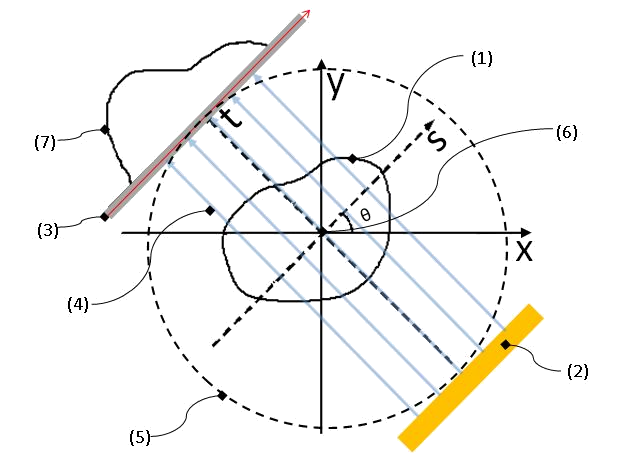
\includegraphics[width=\imsize]{img/CT_PRINCI_PB}
				\source{\href{https://commons.wikimedia.org/wiki/File:CT_PRINCI_PB.jpg}{enwp.org/tomography}}	
		\end{column}
		\begin{column}{0.4\linewidth}
			\begin{enumerate}
				\item Object
				\item Parallel light source
				\item Screen
				\item Transmitted beam
				\item Datum circle
				\item Origin
				\item 1D image
			\end{enumerate}
		\end{column}
	\end{columns}
\end{frame}

\section{Current and ongoing projects}
\begin{frame}{Zebrafish}
	\renewcommand{\imsize}{\paperwidth}%
	\pgfmathsetlength{\imagewidth}{\imsize}%
	\pgfmathsetlength{\imagescale}{\imagewidth/1651}%
	\def\x{1020}% scalebar-x starting at golden ratio of image width of 1651px = 1020
	\def\y{391}% scalebar-y at 90% of image height of 434px = 391
	\makebox[\linewidth]{%
	\begin{tikzpicture}[x=\imagescale,y=-\imagescale]%
		\node[anchor=north west, inner sep=0pt, outer sep=0pt] at (0,0) {\includegraphics[width=\imagewidth]{img/{{zebrafish_rec_voi_side}}}};
		% 1615px = 35.48 > 100px = 2198um > 23px = 500um, 5px = 100um
		%\draw[|-|,blue,thick] (20,154) -- (1634,127) node [sloped,midway,above,fill=white,semitransparent,text opacity=1] {\SI{35.487480000000005}{\milli\meter} (1615px) TEMPORARY!};
		\draw[|-|] (\x,\y) -- (\x+234.19,\y) node [midway,above] {\SI{5}{\milli\meter}};
	\end{tikzpicture}%
	}
	Visualization of a tomographic scan of a zebrafish, fixed in \SI{4}{\percent} PFA.
\end{frame}

\begin{frame}
	\frametitle{Rat head}
	\renewcommand{\imsize}{\paperwidth}%
	\pgfmathsetlength{\imagewidth}{\imsize}%
	\pgfmathsetlength{\imagescale}{\imagewidth/1400}%
	\def\x{865}% scalebar-x starting at golden ratio of image width of 1400px = 865
	\def\y{560}% scalebar-y at 90% of image height of 622px = 560
	\makebox[\linewidth]{%
	\begin{tikzpicture}[x=\imagescale,y=-\imagescale]%
		\node[anchor=north west, inner sep=0pt, outer sep=0pt] at (0,0) {\includegraphics[width=\imagewidth]{./img/{{ratwholehead_rec_side}}}};
		%\spy [red] on (1100,322) in node at (0,0) [anchor=north west];
		% 1358px = 47.76mm > 100px = 3517um > 14px = 500um, 3px = 100um
		%\draw[|-|,blue,thick] (23,291) -- (1380,311) node [sloped,midway,above,fill=white,semitransparent,text opacity=1] {\SI{47.76}{\milli\meter} (1358px) TEMPORARY!};
		\draw[|-|] (\x,\y) -- (\x+140,\y) node [midway,above] {\SI{5}{\milli\meter}};
	\end{tikzpicture}%
	}
	Visualization of a tomographic scan of a rat head, instilled with \uaf and fixed in \SI{4}{\percent} PFA.
\end{frame}

\begin{frame}{Rat brain vessels}
	\renewcommand{\imsize}{\linewidth}%
	\begin{columns}
		\begin{column}{0.618\linewidth}
			\pgfmathsetlength{\imagewidth}{\imsize}%
			\pgfmathsetlength{\imagescale}{\imagewidth/1950}%
			\def\x{1205}% scalebar-x starting at golden ratio of image width of 1950px = 1205
			\def\y{1230}% scalebar-y at 90% of image height of 1367px = 1230
			\begin{tikzpicture}[x=\imagescale,y=-\imagescale]
				\node[anchor=north west, inner sep=0pt, outer sep=0pt] at (0,0) {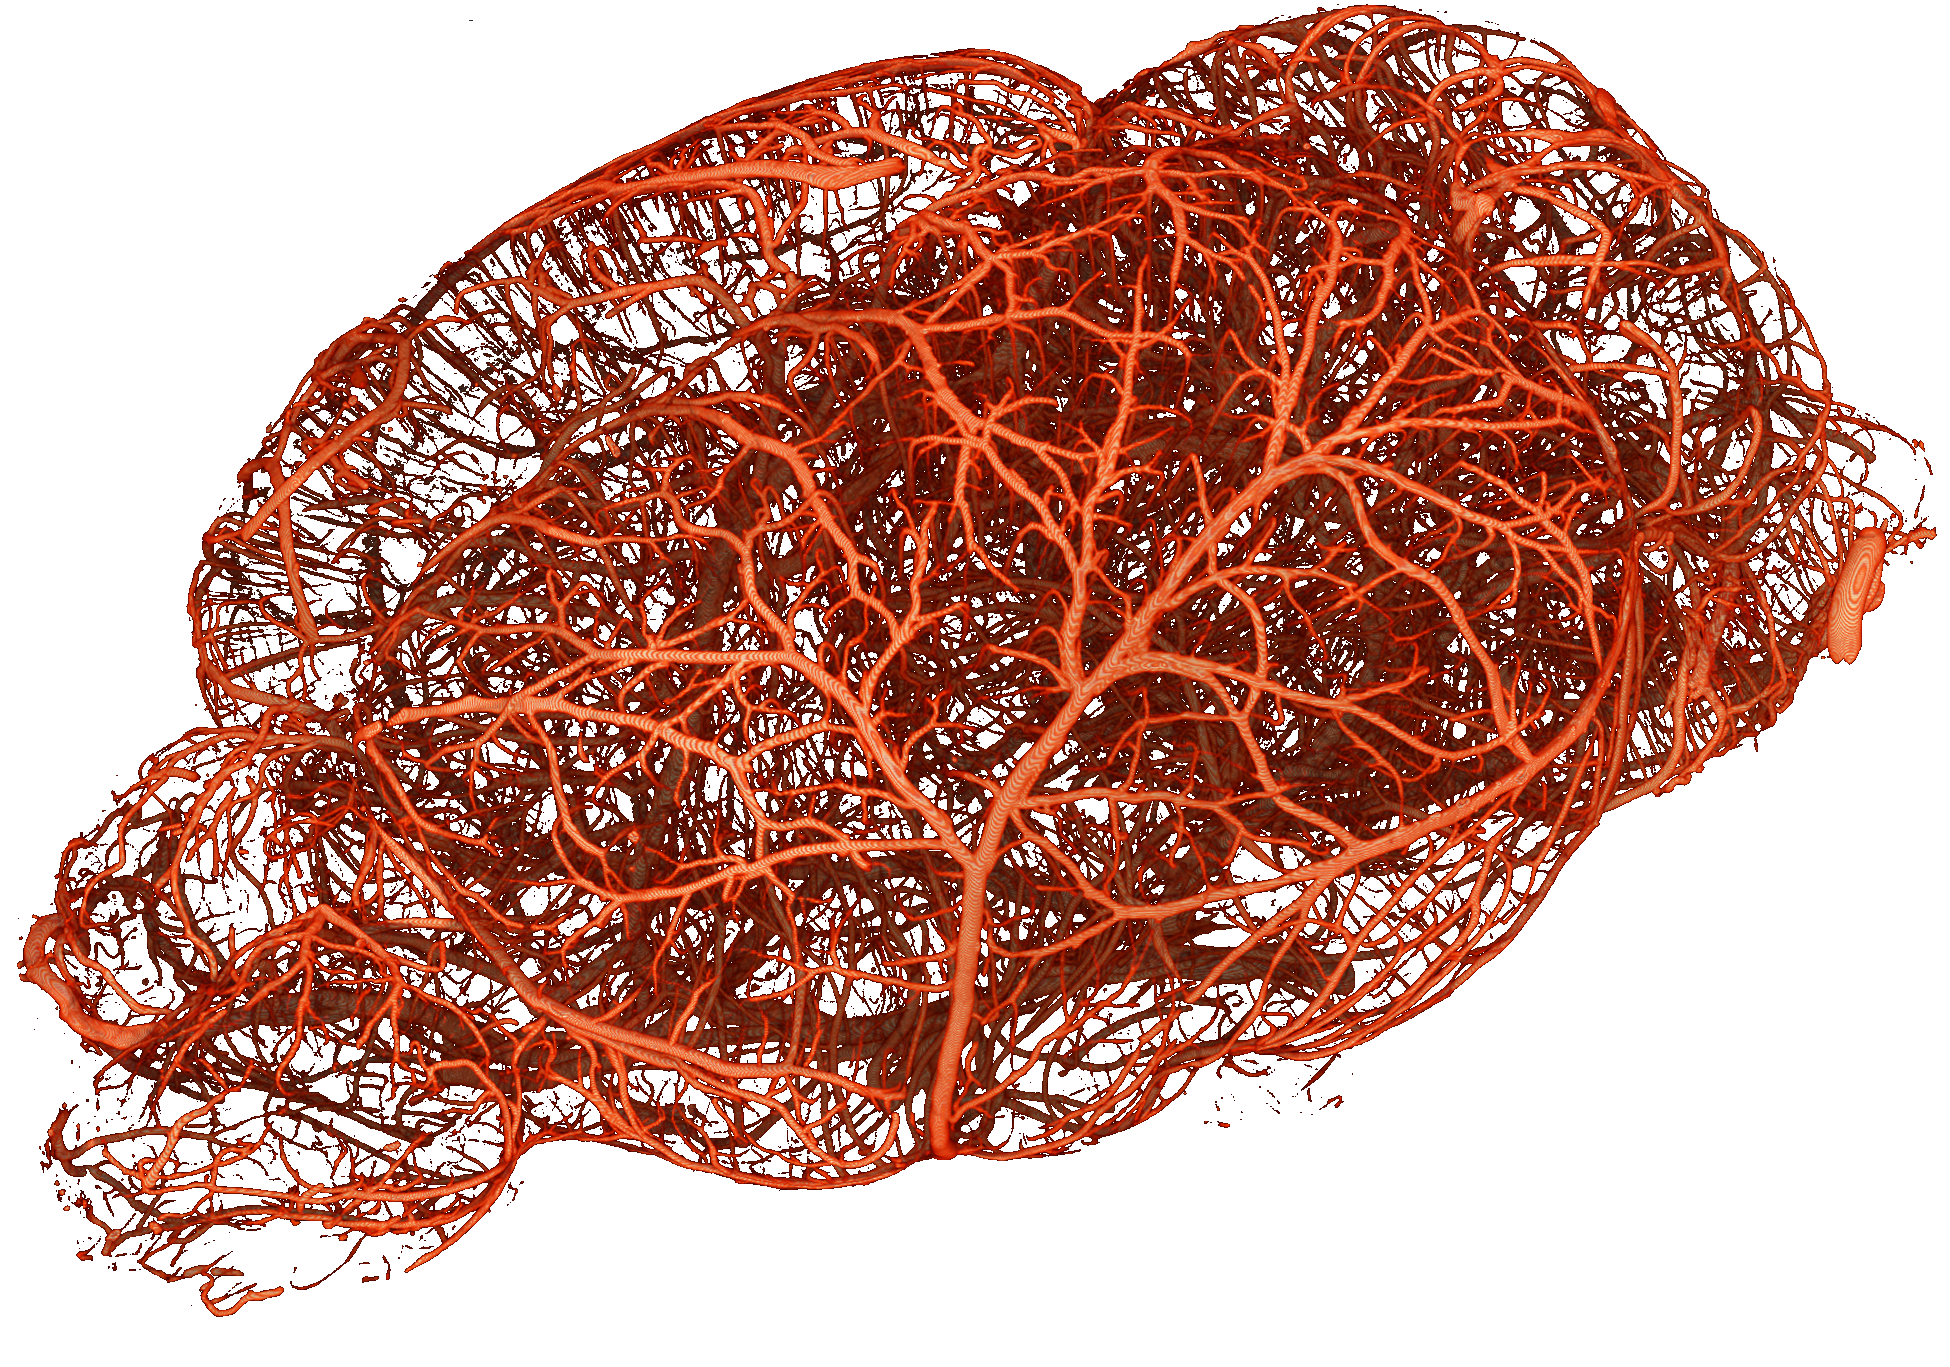
\includegraphics[width=\imagewidth]{img/Ebene_25}};
				% 1949px = 20.0mm > 100px = 1026um > 49px = 500um, 10px = 100um
				%\draw[|-|,blue,thick] (39,1222) -- (1722,239) node [sloped,midway,above,fill=white,semitransparent,text opacity=1] {\SI{20.0}{\milli\meter} (1949px) TEMPORARY!};
				\draw[|-|, thick] (\x,\y) -- (\x+490,\y) node [midway,above] {\SI{5}{\milli\meter}};
				\node [anchor=center] (cb) at (2000,0) {Cerebellum};
				\draw [thick,double,draw=unibe,double=black] (cb.west) to [out=-180, in=0] (1482,144);
				\node [anchor=center] (bs) at (2250,1500) {Brain stem};
				\draw [thick,double,draw=unibe,double=black] (bs.west) to [out=180, in=-45] (1705,725);
				\node [anchor=center, text width=2cm, align=center] (ob) at (550,1500) {Olfactory bulbs};
				\draw [thick,double,draw=unibe,double=black] (ob.west) to [out=180, in=180] (210,880);
				\draw [thick,double,draw=unibe,double=black] (ob.west) to [out=180, in=180] (298,1116);
			\end{tikzpicture}
		\end{column}		
		\begin{column}{0.382\linewidth}
			Visualization of a tomographic scan of a \uaf-filled mouse brain.
		\end{column}
	\end{columns}
\end{frame}

\section{Assessing tumor/metastasis load in lungs}
\begin{frame}
	\frametitle{Tumor metastasis}
	\begin{itemize}
		\item \emph{Problem:} Tumor load?
		\pause
		\item \emph{Solution:} Stereology on \uct data!
		\item[]
		\pause
		\item KP-TNIK mice \cite{DuPage2009} from collaboration with DKF
		\item Stereology as part of \href{https://www.anaintra.unibe.ch/studenten_view.php?filter=aktuell}{Masters Thesis} of \href{http://www.anaweb.ch/ueber_uns/team/detail/index_ger.php?id=485}{Andreas Gübeli}
	\end{itemize}
\end{frame}

\begin{frame}
	\frametitle{Tumor load in lungs, KP-TNIK mice}
	\renewcommand{\imsize}{0.33\linewidth}
	\begin{columns}
		\begin{column}{0.8\linewidth}
			\pgfmathsetlength{\imagewidth}{\imsize}%
			\pgfmathsetlength{\imagescale}{\imagewidth/800}%
			\def\x{494}% scalebar-x starting at golden ratio of image width of 800px = 494
			\def\y{720}% scalebar-y at 90% of image height of 800px = 720
			\begin{tikzpicture}[x=\imagescale,y=-\imagescale]
			\node[anchor=north west, inner sep=0pt, outer sep=0pt] at (0,0) {\includegraphics[width=\imagewidth]{./img/ochsenbein/{{MAX_--11}}}};
			% 800px = 16.0mm > 100px = 2000um > 25px = 500um, 5px = 100um
			%\draw[|-|,blue,thick] (0,400) -- (800,400) node [sloped,midway,above,fill=white,semitransparent,text opacity=1] {\SI{16.0}{\milli\meter} (800px) TEMPORARY!};
			%\draw[|-|] (\x,\y) -- (\x+250,\y) node [midway,above] {\SI{5}{\milli\meter}};
			\end{tikzpicture}%
			\begin{tikzpicture}[x=\imagescale,y=-\imagescale]
			\node[anchor=north west, inner sep=0pt, outer sep=0pt] at (0,0) {\includegraphics[width=\imagewidth]{./img/ochsenbein/{{MAX_--12}}}};
			%\draw[|-|] (\x,\y) -- (\x+250,\y) node [midway,above] {\SI{5}{\milli\meter}};
			\end{tikzpicture}%
			\begin{tikzpicture}[x=\imagescale,y=-\imagescale]
			\node[anchor=north west, inner sep=0pt, outer sep=0pt] at (0,0) {\includegraphics[width=\imagewidth]{./img/ochsenbein/{{MAX_--13}}}};
			\draw[|-|] (\x,\y) -- (\x+250,\y) node [midway,above] {\SI{5}{\milli\meter}};
			\end{tikzpicture}%
			\vspace{0.25cm}%
			\\%
			\begin{tikzpicture}[x=\imagescale,y=-\imagescale]
			\node[anchor=north west, inner sep=0pt, outer sep=0pt] at (0,0) {\includegraphics[width=\imagewidth]{./img/ochsenbein/{{MAX_wt11}}}};
			%\draw[|-|] (\x,\y) -- (\x+250,\y) node [midway,above] {\SI{5}{\milli\meter}};
			\end{tikzpicture}%
			\begin{tikzpicture}[x=\imagescale,y=-\imagescale]
			\node[anchor=north west, inner sep=0pt, outer sep=0pt] at (0,0) {\includegraphics[width=\imagewidth]{./img/ochsenbein/{{MAX_wt12}}}};
			%\draw[|-|] (\x,\y) -- (\x+250,\y) node [midway,above] {\SI{5}{\milli\meter}};
			\end{tikzpicture}%
			\begin{tikzpicture}[x=\imagescale,y=-\imagescale]
			\node[anchor=north west, inner sep=0pt, outer sep=0pt] at (0,0) {\includegraphics[width=\imagewidth]{./img/ochsenbein/{{MAX_wt13}}}};
			\draw[|-|] (\x,\y) -- (\x+250,\y) node [midway,above] {\SI{5}{\milli\meter}};
			\end{tikzpicture}%
		\end{column}
		\begin{column}{0.15\textwidth}
			\begin{itemize}
				\item KO
				\item WT
			\end{itemize}
		\end{column}
	\end{columns}
\end{frame}

\begin{frame}
	\frametitle{Tumor load in lungs, KP-TNIK mice. }
	\renewcommand{\imsize}{\linewidth}%
	\begin{columns}
		\begin{column}{0.8\linewidth}
		\animategraphics[autoplay,palindrome,width=\imsize]{12}{../../Documents/Collaborations/DKF_Lung/movieframes/out-}{001}{255}
		\end{column}
		\begin{column}{0.15\textwidth}
			\begin{itemize}
				\item KO
				\item WT
			\end{itemize}
		\end{column}
	\end{columns}
\end{frame}

\section{Lung fibrosis}
\begin{frame}
	\frametitle{Backstory}
	\begin{itemize}
		\item \emph{Problem:} Lung fibrosis grading \cite{Ashcroft1988a} and correct sampling for proper assessment?
		\pause
		\item \emph{Solution:} \uct!
		\item[]
		\pause
	\item \uct is a tool to help grade fibrosis \cite{DeLanghe2012,Rodt2010}
		\begin{itemize}
			\item Detect and grade fibrosis
			\item Get indications where to perform the sampling
			\item But still limited resolution!
		\end{itemize}
	\end{itemize}
\end{frame}

\begin{frame}
	\frametitle{Multimodal imaging: \uct and 3View, correlated imaging}
	\renewcommand{\imsize}{0.25\linewidth}
	\begin{itemize}
		\item Fibrose grading should be done on ultra fine level \cite{Hubner2008}
		\pause
		\item \uct combined with serial block-face scanning electron microscopy (\href{http://www.gatan.com/products/sem-imaging-spectroscopy/3view-system}{3View})
		\item Registration of datasets, from overview to ultrafine structure
		\item Combination with histology
		\pause
		\item Multimodal has been done before, with luck and not in 3D :) \cite{Haberthuer2009}
	\end{itemize}
\end{frame}

\begin{frame}
	\frametitle{Overview scan with \SI{20}{\micro\meter} pixel size}
	\renewcommand{\imsize}{0.53\linewidth}
	\pgfmathsetlength{\imagewidth}{\imsize}%
	\pgfmathsetlength{\imagescale}{\imagewidth/993}%
	\def\x{614}% scalebar-x starting at golden ratio of image width of 993px = 614
	\def\y{859}% scalebar-y at 90% of image height of 954px = 859
	\begin{tikzpicture}[x=\imagescale,y=-\imagescale]
		\node[anchor=north west, inner sep=0pt, outer sep=0pt] at (0,0) {\animategraphics[autoplay, palindrome, width=\imsize]{24}{./img/movie_tumor_20um/mouse_tumor_rec0}{001}{461}};
		% 698px = 16.12mm > 100px = 2309um > 22px = 500um, 4px = 100um
		%\draw[|-|,blue,thick] (89,571) -- (787,576) node [sloped,midway,above,fill=white,semitransparent,text opacity=1] {\SI{16.12}{\milli\meter} (806px) TEMPORARY!};
		\draw[|-|, thick] (\x,\y) -- (\x+217,\y) node [midway,above] {\SI{5}{\milli\meter}};
	\end{tikzpicture}%
\end{frame}

\begin{frame}[label=current]
	\frametitle{Overview, Detail and 3View}
	\renewcommand{\imsize}{0.5\linewidth}
	\pgfmathsetlength{\imagewidth}{\imsize}%
	\pgfmathsetlength{\imagescale}{\imagewidth/7776}%
	\def\x{4806}% scalebar-x starting at golden ratio of image width of 7776px = 4806
	\def\y{6998}% scalebar-y at 90% of image height of 7776px = 6998
	\begin{tikzpicture}[x=\imagescale,y=-\imagescale,remember picture]
		\node[anchor=north west, inner sep=0pt, outer sep=0pt] at (0,0) {\includegraphics[width=\imagewidth]{./img/fibrosis/Mouse_Tumor_IR_rec00001610}};
		% 7776px = 23.328mm > 100px = 300um > 167px = 500um, 33px = 100um
		%\draw[|-|,blue,thick] (0,3888) -- (7776,3888) node [sloped,midway,above,fill=white,semitransparent,text opacity=1] {\SI{23.328}{\milli\meter} (7776px) TEMPORARY!};
		\draw[|-|,white,thick] (\x,\y) -- (\x+1670,\y) node [midway,above] {\SI{5}{\milli\meter}};
		\node<3>[red,draw,circle,inner sep=6pt] (overview) at (1500,4160) {};
	\end{tikzpicture}%
	\pause
	\pgfmathsetlength{\imagewidth}{\imsize}%
	\pgfmathsetlength{\imagescale}{\imagewidth/3812}%
	\def\x{2356}% scalebar-x starting at golden ratio of image width of 3812px = 2356
	\def\y{3431}% scalebar-y at 90% of image height of 3812px = 3431
	\begin{tikzpicture}[x=\imagescale,y=-\imagescale, remember picture]
		\node<2->[anchor=north west, inner sep=0pt, outer sep=0pt] at (0,0) {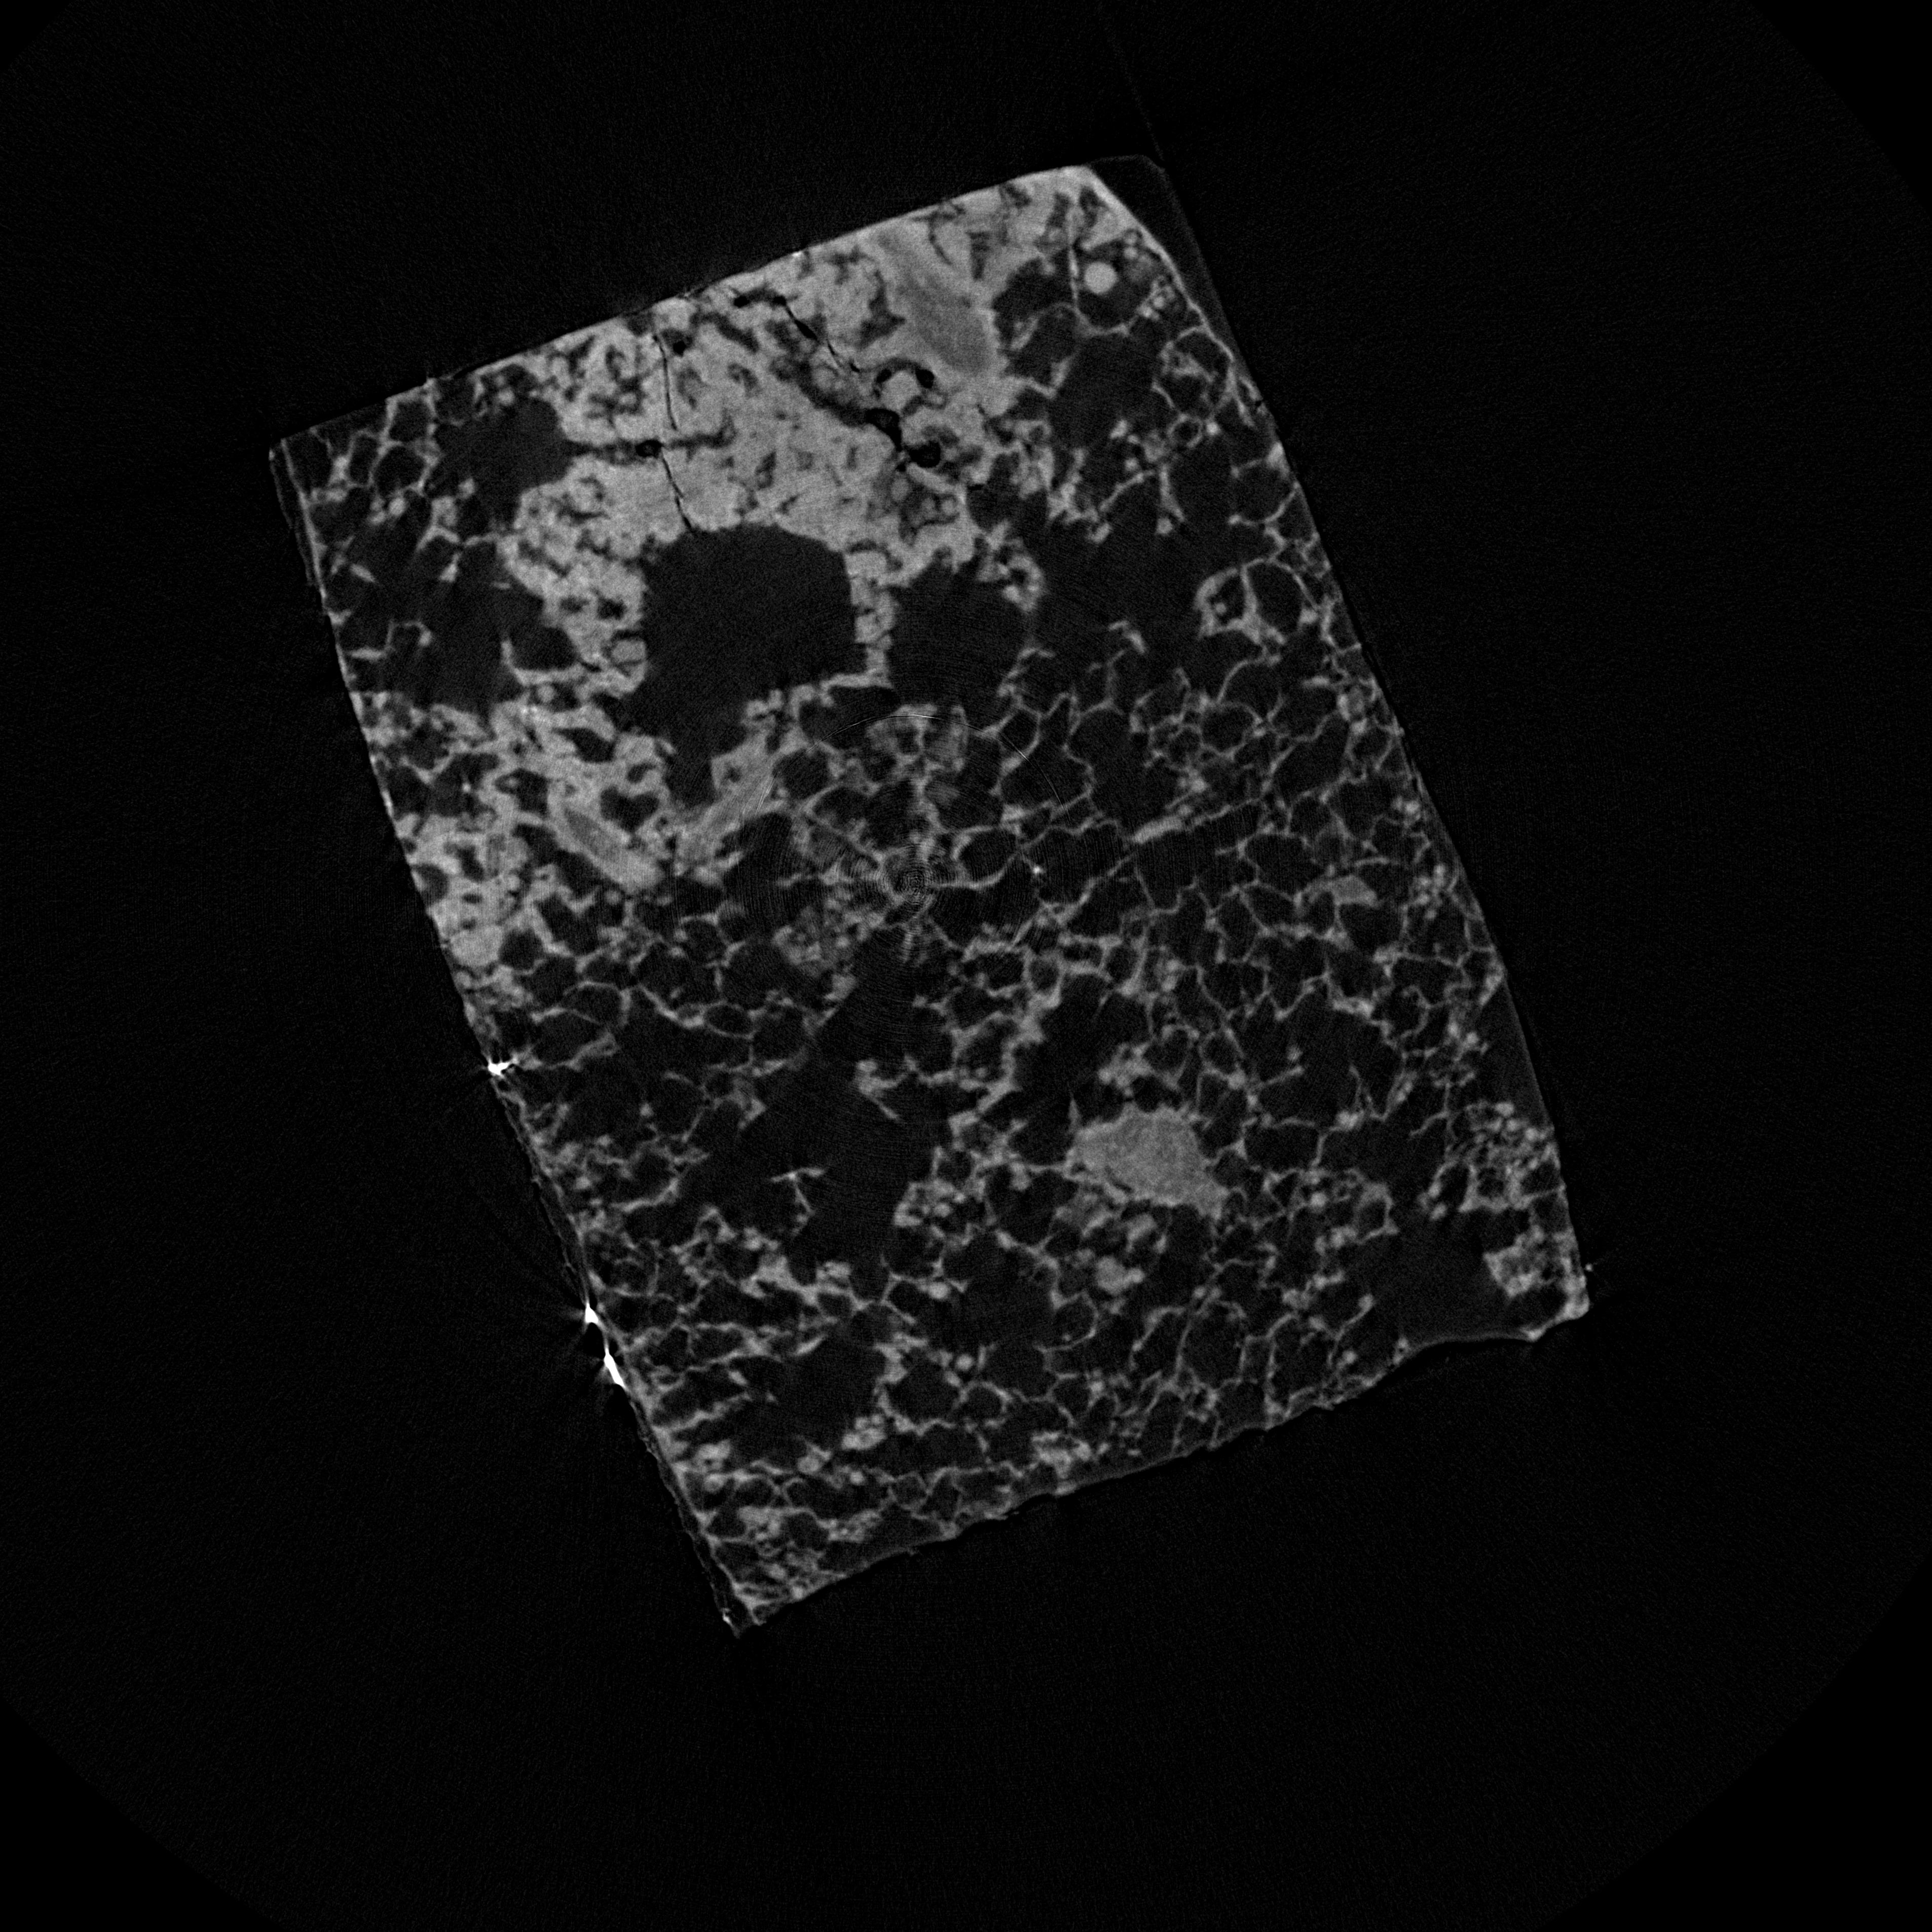
\includegraphics[width=\imagewidth]{./img/fibrosis/uct_Cube}};
		%\spy [red] on (3512,3512) in node at (0,0) [anchor=north west];
		% 3812px = 1.906mm > 100px = 50um > 1000px = 500um, 200px = 100um
		%\draw[|-|,blue,thick] (0,1906) -- (3812,1906) node [sloped,midway,above,fill=white,semitransparent,text opacity=1] {\SI{1.906}{\milli\meter} (3812px) TEMPORARY!};
		\draw[|-|,white,thick] (\x,\y) -- (\x+1000,\y) node [midway,above] {\SI{500}{\micro\meter}};
		\node<3> (detail-1) at (2124,336) {};
		\node<3> (detail-2) at (1470,3222) {};
	\end{tikzpicture}%
	\begin{tikzpicture}[remember picture,overlay]
		\draw<3>[dashed,red] (overview) -- (detail-1);
		\draw<3>[dashed,red] (overview) -- (detail-2);
	\end{tikzpicture}
\end{frame}

\begin{frame}[label=current]
	\frametitle{Overview, Detail and 3View}
	\renewcommand{\imsize}{0.5\linewidth}
	\pgfmathsetlength{\imagewidth}{\imsize}%
	\pgfmathsetlength{\imagescale}{\imagewidth/8192}%
	\def\x{5063}% scalebar-x starting at golden ratio of image width of 8192px = 5063
	\def\y{6313}% scalebar-y at 90% of image height of 7014px = 6313
	\begin{tikzpicture}[x=\imagescale,y=-\imagescale]
		\node[anchor=north west, inner sep=0pt, outer sep=0pt] at (0,0) {\includegraphics[width=\imagewidth]{./img/fibrosis/3View_Overview}};
	% 8192px = 0.9486336mm > 100px = 12um > 4318px = 500um, 864px = 100um
	%\draw[|-|,blue,thick] (0,3507) -- (8192,3507) node [sloped,midway,above,fill=white,semitransparent,text opacity=1] {\SI{0.9486336}{\milli\meter} (8192px) TEMPORARY!};
	\draw[|-|,white,thick] (\x,\y) -- (\x+864,\y) node [midway,above] {\SI{100}{\micro\meter}};
\end{tikzpicture}%
	\pause
\pgfmathsetlength{\imagewidth}{\imsize}%
\pgfmathsetlength{\imagescale}{\imagewidth/8192}%
\def\x{5063}% scalebar-x starting at golden ratio of image width of 8192px = 5063
\def\y{7373}% scalebar-y at 90% of image height of 8192px = 7373
\begin{tikzpicture}[x=\imagescale,y=-\imagescale]
		\node[anchor=north west, inner sep=0pt, outer sep=0pt] at (0,0) {\includegraphics[width=\imagewidth]{./img/fibrosis/3View_Detail}};;
	% 8192px = 0.098304mm > 100px = 1um > 41667px = 500um, 8333px = 100um
	%\draw[|-|,blue,thick] (0,4096) -- (8192,4096) node [sloped,midway,above,fill=white,semitransparent,text opacity=1] {\SI{0.098304}{\milli\meter} (8192px) TEMPORARY!};
	\draw[|-|,white,thick] (\x,\y) -- (\x+833.3,\y) node [midway,above] {\SI{10}{\micro\meter}};
\end{tikzpicture}%
\end{frame}

\begin{frame}[label=current]
	\frametitle{Overview, Detail and 3View}
	\renewcommand{\imsize}{0.6\linewidth}
	\pgfmathsetlength{\imagewidth}{\imsize}%
	\pgfmathsetlength{\imagescale}{\imagewidth/8192}%
	\def\x{5063}% scalebar-x starting at golden ratio of image width of 8192px = 5063
	\def\y{6313}% scalebar-y at 90% of image height of 7014px = 6313
	\begin{tikzpicture}[x=\imagescale,y=-\imagescale]
		\node[anchor=north west, inner sep=0pt, outer sep=0pt] at (0,0) {\includegraphics[width=\imagewidth]{./img/fibrosis/3View_Registration}};
		% 8192px = 0.9486336mm > 100px = 12um > 4318px = 500um, 864px = 100um
		%\draw[|-|,blue,thick] (0,3507) -- (8192,3507) node [sloped,midway,above,fill=white,semitransparent,text opacity=1] {\SI{0.9486336}{\milli\meter} (8192px) TEMPORARY!};
		\draw[|-|,white,thick] (\x,\y) -- (\x+864,\y) node [midway,above] {\SI{100}{\micro\meter}};
	\end{tikzpicture}%
\end{frame}

\begin{frame}[label=current]
	\frametitle{Overview, Detail and 3View}
	\renewcommand{\imsize}{0.5\linewidth}
	\pgfmathsetlength{\imagewidth}{\imsize}%
	\pgfmathsetlength{\imagescale}{\imagewidth/3812}%
	\def\x{2356}% scalebar-x starting at golden ratio of image width of 3812px = 2356
	\def\y{3431}% scalebar-y at 90% of image height of 3812px = 3431
	\begin{tikzpicture}[x=\imagescale,y=-\imagescale]
		\node[anchor=north west, inner sep=0pt, outer sep=0pt] at (0,0) {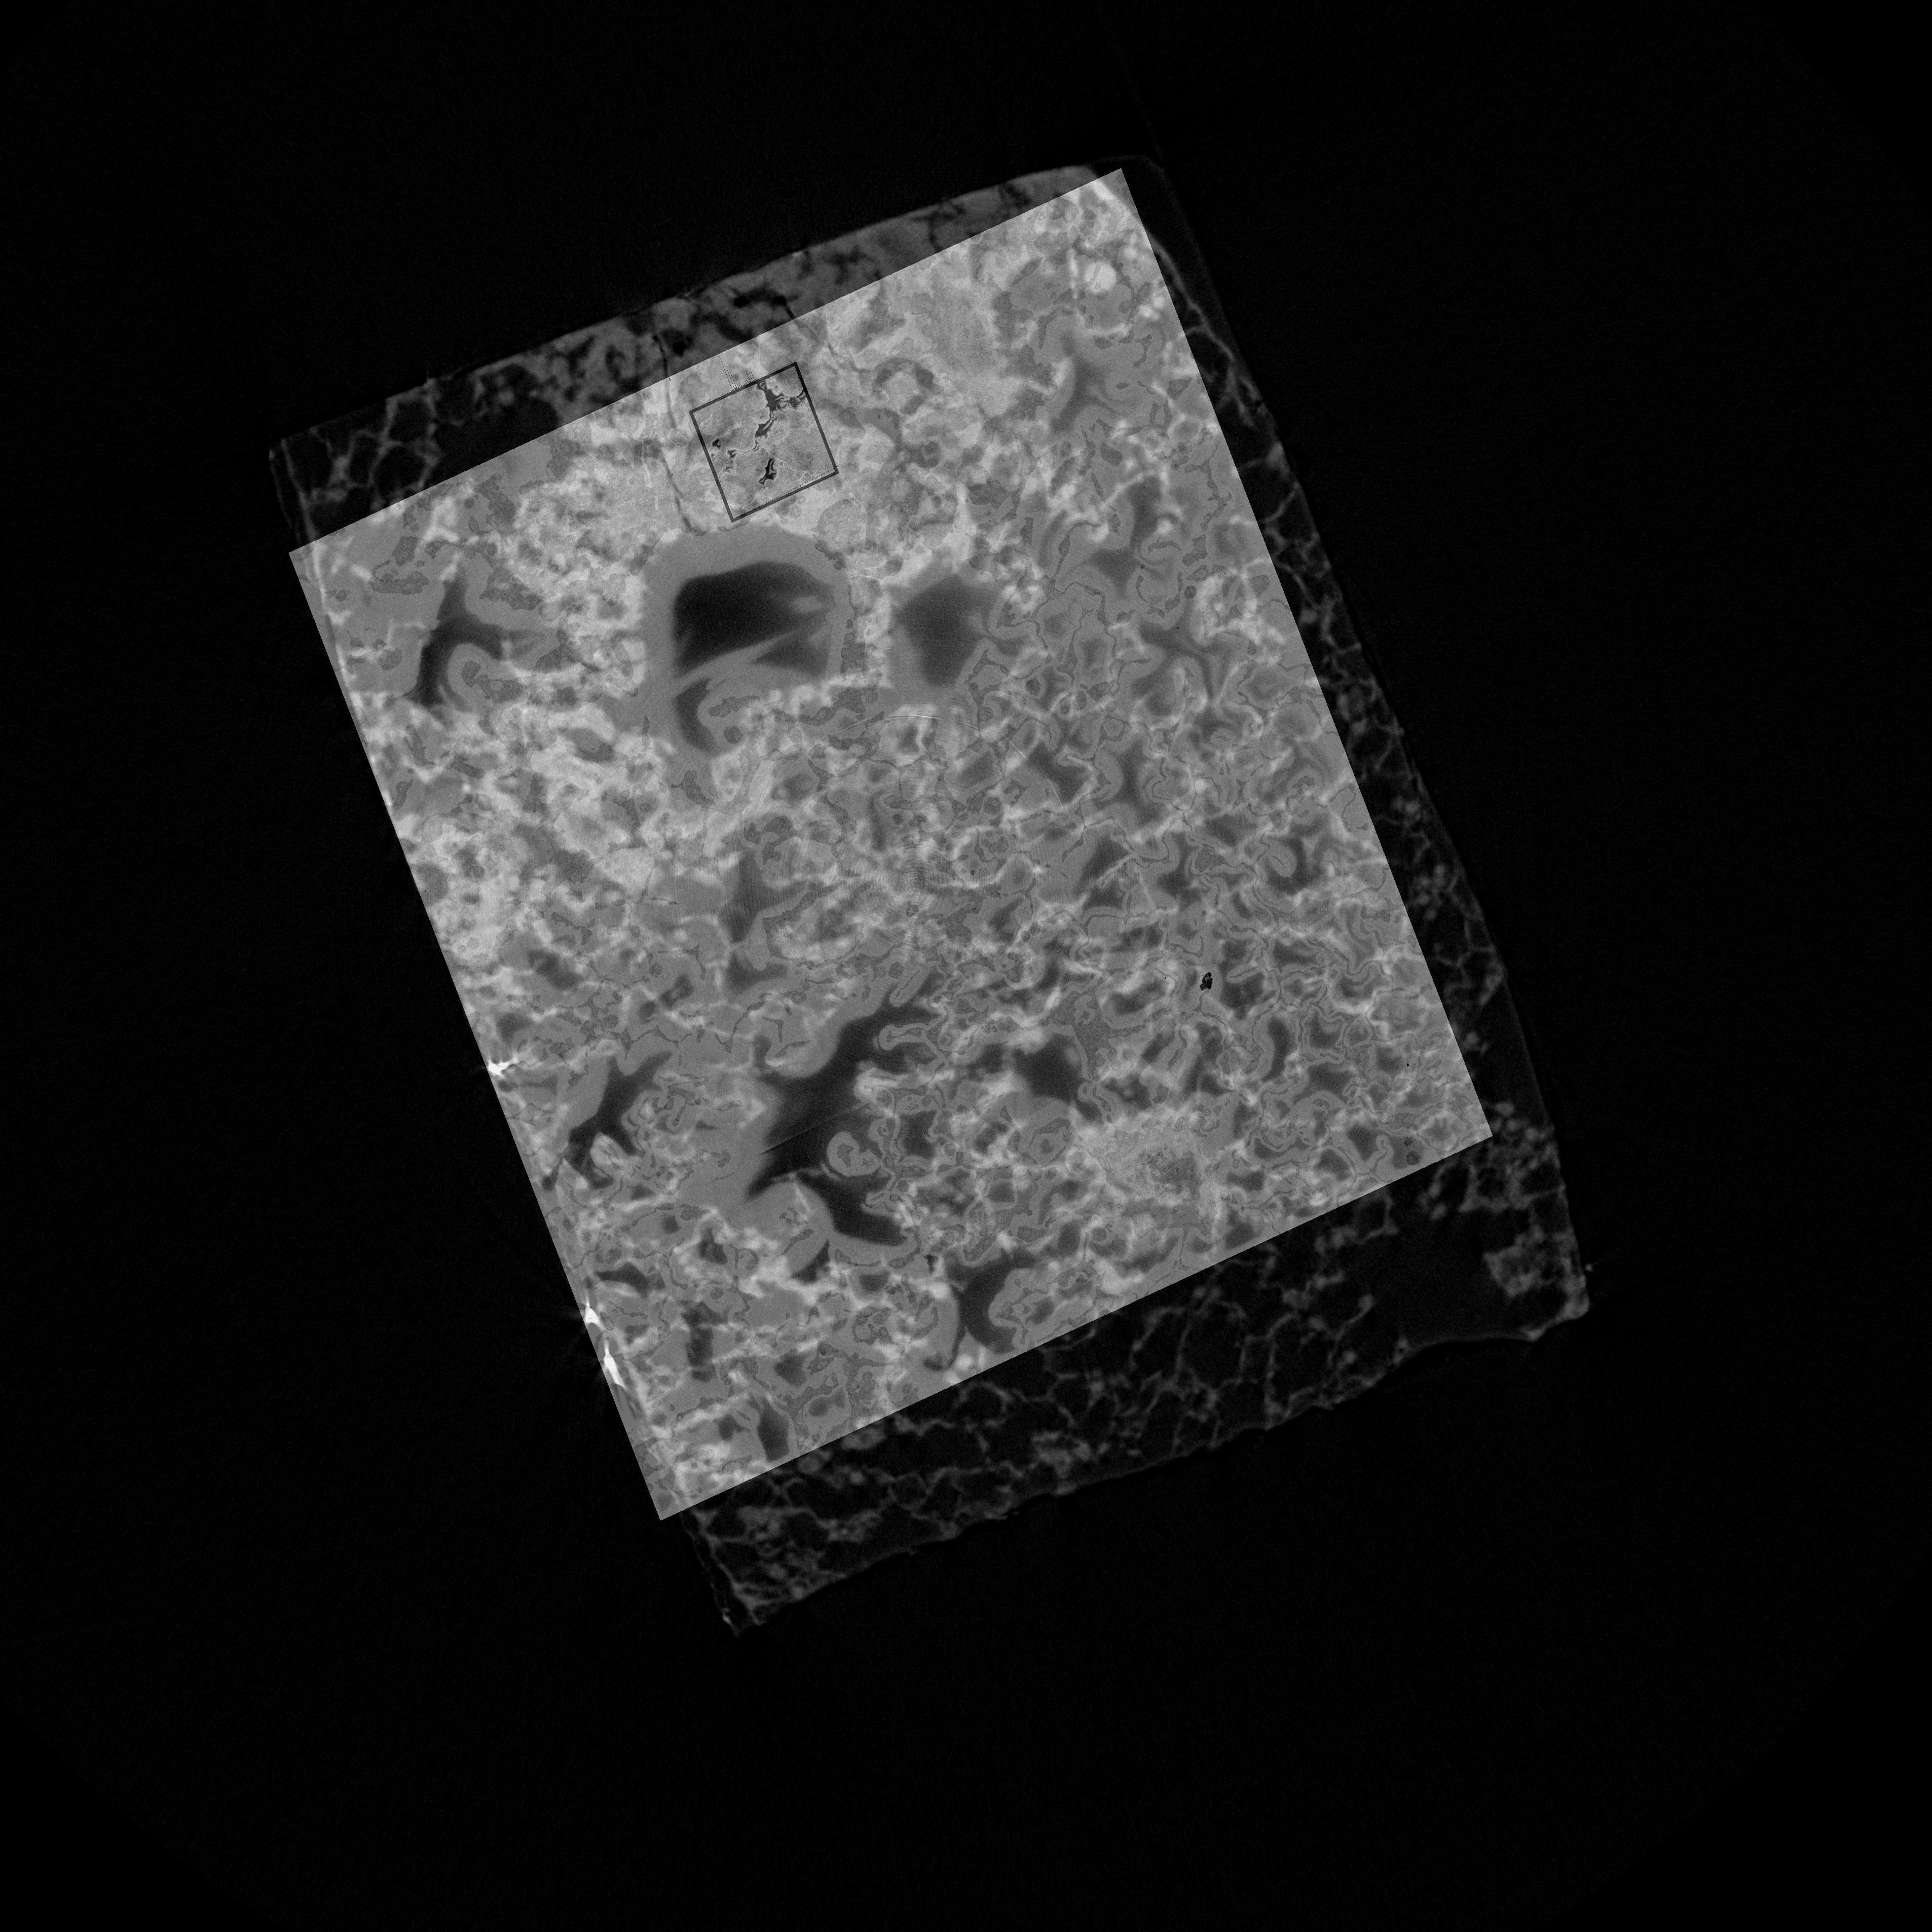
\includegraphics[width=\imagewidth]{./img/fibrosis/uCT_Cube_with_3View_Registration_Average}};
		% 3812px = 11.436mm > 100px = 300um > 167px = 500um, 33px = 100um
		%\draw[|-|,blue,thick] (0,1906) -- (3812,1906) node [sloped,midway,above,fill=white,semitransparent,text opacity=1] {\SI{11.436}{\milli\meter} (3812px) TEMPORARY!};
	\draw[|-|,white,thick] (\x,\y) -- (\x+167,\y) node [midway,above] {\SI{500}{\micro\meter}};
	\end{tikzpicture}%
\end{frame}

\section{Assessing brain tumors nondestructively}
\label{sec:grenoble}
\begin{frame}
	\frametitle{Brain tumor radiation treatment}
	\begin{itemize}
		\item \emph{Problem:} Tumor angiogenesis/radiation therapy?
		\pause
		\item \emph{Solution:} Nondestructive imaging and assessment with \uct!
		\item[]
		\pause
		\item Judah Folkman: \blockquote[\cite{Sherwood1971}]{Tumors that exist in the dormant state have not become vascularised.}
		\pause
		\item Antiangiogenesis as tumor therapy
		\begin{itemize}
			\item \href{https://clinicaltrials.gov/ct2/results?term=antiangiogenic}{\textgreater4000 clinical trials}
			\item Results disappointing
			\item New, powerful and simple treatment strategies are needed
		\end{itemize}
		\pause
		\item Microbeam radiation therapy
		\begin{itemize}
			\item Delivery of very high dose (\SIrange{100}{5000}{\gray}) in less than \SI{1}{\second}.
			\item \emph{Excellent} survival rate \cite{Laissue1998}
		\end{itemize}
	\end{itemize}
\end{frame}

\begin{frame}
	\frametitle{Rat brain tumors}
	\begin{columns}
		\begin{column}{0.5\linewidth}
			\begin{itemize}
		    	\item Induced tumors
		    	\item 9L Gliosarcoma \cite{Bouchet2014}
		    	\item Microbeam and broadbeam treatment vs.\ control
		    	\item \uaf-filled brain vasculature
		    	\item Nondestructive extraction of
		    	\begin{itemize}
		    		\item Vessel to tumor volume ratio
		    		\item Vessel surface
		    		\item Intra-tumoral microvessel density (IMD, \cite{Hasan2002})
		    	\end{itemize}
			\end{itemize}
		\end{column}
		\renewcommand{\imsize}{1\linewidth}
		\begin{column}{0.28\linewidth}
			\pgfmathsetlength{\imagewidth}{\imsize}%
			\pgfmathsetlength{\imagescale}{\imagewidth/299}%
			\def\x{185}% scalebar-x starting at golden ratio of image width of 299px = 185
			\def\y{460}% scalebar-y at 90% of image height of 546px = 491
			\begin{tikzpicture}[x=\imagescale,y=-\imagescale]
				\node[anchor=north west, inner sep=0pt, outer sep=0pt] at (0,0) {\includegraphics[width=\imagewidth]{./img/{{macro_brain_d24_ctrl}}}};
				% 500px = 30.0mm > 100px = 6004um > 8px = 500um, 2px = 100um
				%\draw[|-|,blue,thick] (179,523) -- (121,27) node [sloped,midway,above,fill=white,semitransparent,text opacity=1] {\SI{30.0}{\milli\meter} (500px) TEMPORARY!};
				\draw[|-|] (\x,\y) -- (\x+83,\y) node [midway,above] {\SI{5}{\milli\meter}};
				\pause
				\draw<2>[red, thick] (203,192) circle (50);
			\end{tikzpicture}%
		\end{column}
		\begin{column}{0.28\linewidth}
			\pgfmathsetlength{\imagewidth}{\imsize}%
			\pgfmathsetlength{\imagescale}{\imagewidth/299}%
			\def\x{185}% scalebar-x starting at golden ratio of image width of 299px = 185
			\def\y{460}% scalebar-y at 90% of image height of 511px = 460
			\begin{tikzpicture}[x=\imagescale,y=-\imagescale]
				\node[anchor=north west, inner sep=0pt, outer sep=0pt] at (0,0) {\includegraphics[width=\imagewidth]{./img/{{macro_brain_d24_mrt}}}};
				% 463px = 30.0mm > 100px = 6478um > 8px = 500um, 2px = 100um
				%\draw[|-|,blue,thick] (163,479) -- (162,16) node [sloped,midway,above,fill=white,semitransparent,text opacity=1] {\SI{30.0}{\milli\meter} (463px) TEMPORARY!};
				\draw[|-|] (\x,\y) -- (\x+77,\y) node [midway,above] {\SI{5}{\milli\meter}};
				\draw<2>[red, thick] (199,187) circle (30);
			\end{tikzpicture}%
		\end{column}		
	\end{columns}	
\end{frame}

\begin{frame}
	\frametitle{Rat brain tumors}
	\begin{itemize}
		\item Scan (\SI{18}{\hour})
		\item Reconstruct (\SIrange{2}{4}{\hour})
		\item Delineate ROI (\SI{1}{\hour})
		\item Threshold
		\item Calculate Tumor and vessel volume
	\end{itemize}
\end{frame}

\begin{frame}
	\frametitle{Rat brain tumors}
	\renewcommand{\imsize}{\linewidth}
	\begin{columns}
		\begin{column}{0.33\paperwidth}
			\animategraphics[autoplay,palindrome,width=\imsize]{12}{./img/movie_b09/b09_ctrl_d24t14_0}{001}{341}
			\centering Control
		\end{column}
		\begin{column}{0.33\paperwidth}
			\animategraphics[autoplay,palindrome,width=\imsize]{12}{./img/movie_b18/b18_mrt_d24t14_0}{001}{341}
		\centering Microbeam
		\end{column}
		\begin{column}{0.33\paperwidth}
			\animategraphics[autoplay,palindrome,width=\imsize]{12}{./img/movie_b68/b68_bb_d24t14_0}{001}{341}
		\centering Broadbeam
		\end{column}
	\end{columns}
\end{frame}

\renewcommand{\imsize}{0.8\textheight}
\begin{frame}
	\frametitle{Tumor volume}
	\includegraphics[height=\imsize]{../../Documents/Brain-Grenoble/fig/tumor_volume}
\end{frame}

\begin{frame}
	\frametitle{Tumor volume}
	\includegraphics[height=\imsize]{../../Documents/Brain-Grenoble/fig/tumor_volume_day}
\end{frame}

\begin{frame}
	\frametitle{Vessel ratio}
	\includegraphics[height=\imsize]{../../Documents/Brain-Grenoble/fig/vessel_vol_per_tumor_volume}
\end{frame}

\begin{frame}
	\frametitle{Vessel ratio}
	\includegraphics[height=\imsize]{../../Documents/Brain-Grenoble/fig/vessel_vol_per_tumor_volume_day}
\end{frame}

\begin{frame}
	\frametitle{Thanks}
	\begin{itemize}
		\item Topographic and clinical Anatomy
		\item Audrey Bouchet
		\item Jean Laissue
		\item ESRF Grenoble
		\item SNF
		\pause
		\item You, for listening
		\pause
		\item Questions?
	\end{itemize}
\end{frame}

\begin{frame}[allowframebreaks]
	\frametitle{References}
	\renewcommand*{\bibfont}{\tiny}
	\setbeamertemplate{bibliography item}{\insertbiblabel}
	\printbibliography
\end{frame}

\end{document}
